\documentclass[11pt,a4paper]{article}
\usepackage[margin=2.5cm]{geometry}
\usepackage{enumitem}
\usepackage{titlesec}
\usepackage{hyperref}
\usepackage{xcolor}
\usepackage{booktabs}
\usepackage{parskip}
\usepackage{graphicx}
\usepackage{amsmath}
\usepackage{float}
\usepackage{listings}
\usepackage{tcolorbox}
\tcbuselibrary{listings,breakable,skins}

\definecolor{accent}{RGB}{30,70,120}
\definecolor{green}{RGB}{40,120,40}
\definecolor{red}{RGB}{180,40,40}
\definecolor{codebg}{RGB}{245,245,245}
\definecolor{codeframe}{RGB}{200,200,200}
\definecolor{codekw}{RGB}{0,100,170}
\definecolor{codecomment}{RGB}{100,130,100}
\definecolor{codestr}{RGB}{170,55,55}
\definecolor{strongbg}{RGB}{230,245,230}
\definecolor{strongframe}{RGB}{60,140,60}
\definecolor{warnbg}{RGB}{255,250,230}
\definecolor{warnframe}{RGB}{180,150,40}
\definecolor{failbg}{RGB}{255,235,235}
\definecolor{failframe}{RGB}{180,60,60}

\newtcolorbox{resultbox}[2][]{
    enhanced,
    colback=#2bg,
    colframe=#2frame,
    boxrule=0.8pt,
    arc=3pt,
    left=6pt, right=6pt, top=4pt, bottom=4pt,
    fonttitle=\bfseries\color{#2frame},
    title={#1},
    breakable,
}

\lstdefinestyle{python}{
    language=Python,
    basicstyle=\ttfamily\footnotesize,
    keywordstyle=\color{codekw}\bfseries,
    commentstyle=\color{codecomment}\itshape,
    stringstyle=\color{codestr},
    showstringspaces=false,
    breaklines=true,
    breakatwhitespace=true,
    tabsize=4,
    numbers=left,
    numberstyle=\tiny\color{gray},
    numbersep=8pt,
}

\lstdefinestyle{shell}{
    language=bash,
    basicstyle=\ttfamily\footnotesize,
    keywordstyle=\color{codekw},
    commentstyle=\color{codecomment}\itshape,
    showstringspaces=false,
    breaklines=true,
    tabsize=4,
    numbers=none,
}

\newtcolorbox{codebox}[1][]{
    colback=codebg,
    colframe=codeframe,
    boxrule=0.5pt,
    arc=2pt,
    left=2pt, right=2pt, top=2pt, bottom=2pt,
    breakable,
    title={\small\ttfamily #1},
    fonttitle=\bfseries\color{accent},
}

\titleformat{\section}{\large\bfseries\color{accent}}{}{0em}{}[\titlerule]
\titleformat{\subsection}{\normalsize\bfseries\color{accent}}{}{0em}{}

\hypersetup{colorlinks=true, linkcolor=accent, urlcolor=accent}

\begin{document}

% ══════════════════════════════════════════════════════════════════
% TITLE
% ══════════════════════════════════════════════════════════════════

\begin{center}
\vspace*{2cm}
{\Huge\bfseries\color{accent} The Recycling Portfolio}\\[1em]
{\LARGE Momentum Timing Across\\[0.3em]
Bitcoin, Copper, and Natural Gas}\\[2em]
{\large Robin Langer}\\[0.5em]
{\small August 2026}\\[3em]
\textit{``When one asset says `sit out,' put the money\\
where another asset says `get in.'\,''}
\vspace*{1.5cm}
\end{center}

\thispagestyle{empty}



% ══════════════════════════════════════════════════════════════════
% HEADLINE
% ══════════════════════════════════════════════════════════════════

\begin{resultbox}[]{warn}
\begin{center}
\Large\bfseries \$10,000 invested five years ago $\longrightarrow$ \$108,003 today.
\end{center}
\end{resultbox}

% ══════════════════════════════════════════════════════════════════
% WHY THESE THREE
% ══════════════════════════════════════════════════════════════════

\section*{Why These Three?}

\begin{resultbox}[Diversification]{strong}
The daily strategy returns of the three assets have near-zero
correlation:

\vspace{0.3em}
\begin{tabular}{@{}lccc@{}}
    \toprule
    & \textbf{BTC} & \textbf{Copper} & \textbf{NatGas} \\
    \midrule
    BTC     & 1.000 & --- & --- \\
    Copper  & 0.056 & 1.000 & --- \\
    NatGas  & 0.017 & $-0.032$ & 1.000 \\
    \bottomrule
\end{tabular}

\vspace{0.5em}
Near-zero correlation means that when one asset is active, the
others usually aren't. Over the 5-year period, all three are active
simultaneously on only \textbf{2\% of days}. This is portfolio
diversification at its best: the assets take turns using the capital.
\end{resultbox}






% ══════════════════════════════════════════════════════════════════
% THE THREE ASSETS
% ══════════════════════════════════════════════════════════════════

\section{The Three Assets}

Each asset was selected from a broader cross-asset study (see
\textit{The Bookmaker's Edge}) based on three criteria: strong
momentum alpha, reliable volume data, and low correlation with
the other assets.

\subsection{Bitcoin (BTC-USD, 180-day lookback)}

The flagship. The bookmaker model produces its strongest and most
consistent signal on Bitcoin.

\vspace{0.5em}
\begin{tabular}{@{}lr@{}}
    \toprule
    \textbf{Metric} & \textbf{Value} \\
    \midrule
    Strategy return    & $+462.7\%$ \\
    Buy \& hold return & $+167.5\%$ \\
    Alpha              & \textcolor{green}{\textbf{+295.2\%}} \\
    Sharpe ratio       & $1.16$ \\
    Max drawdown       & $-28.1\%$ (vs $-76.6\%$ buy \& hold) \\
    Win rate           & 62\% (16 trades) \\
    Win/loss ratio     & 14:1 ($+26.8\%$ avg win vs $-1.9\%$ avg loss) \\
    Days in asset      & 34\% \\
    \bottomrule
\end{tabular}

\vspace{0.5em}
\begin{tcolorbox}[colback=blue!5, colframe=blue!40, boxrule=0.5pt, arc=3pt,
    left=6pt, right=6pt, top=4pt, bottom=4pt]
{\small\textit{The Sharpe ratio measures return per unit of risk:
average return divided by its volatility, annualised.
Above 1.0 is strong; it means each unit of uncertainty
is rewarded with more than one unit of return.}}
\end{tcolorbox}

\begin{figure}[H]
    \centering
    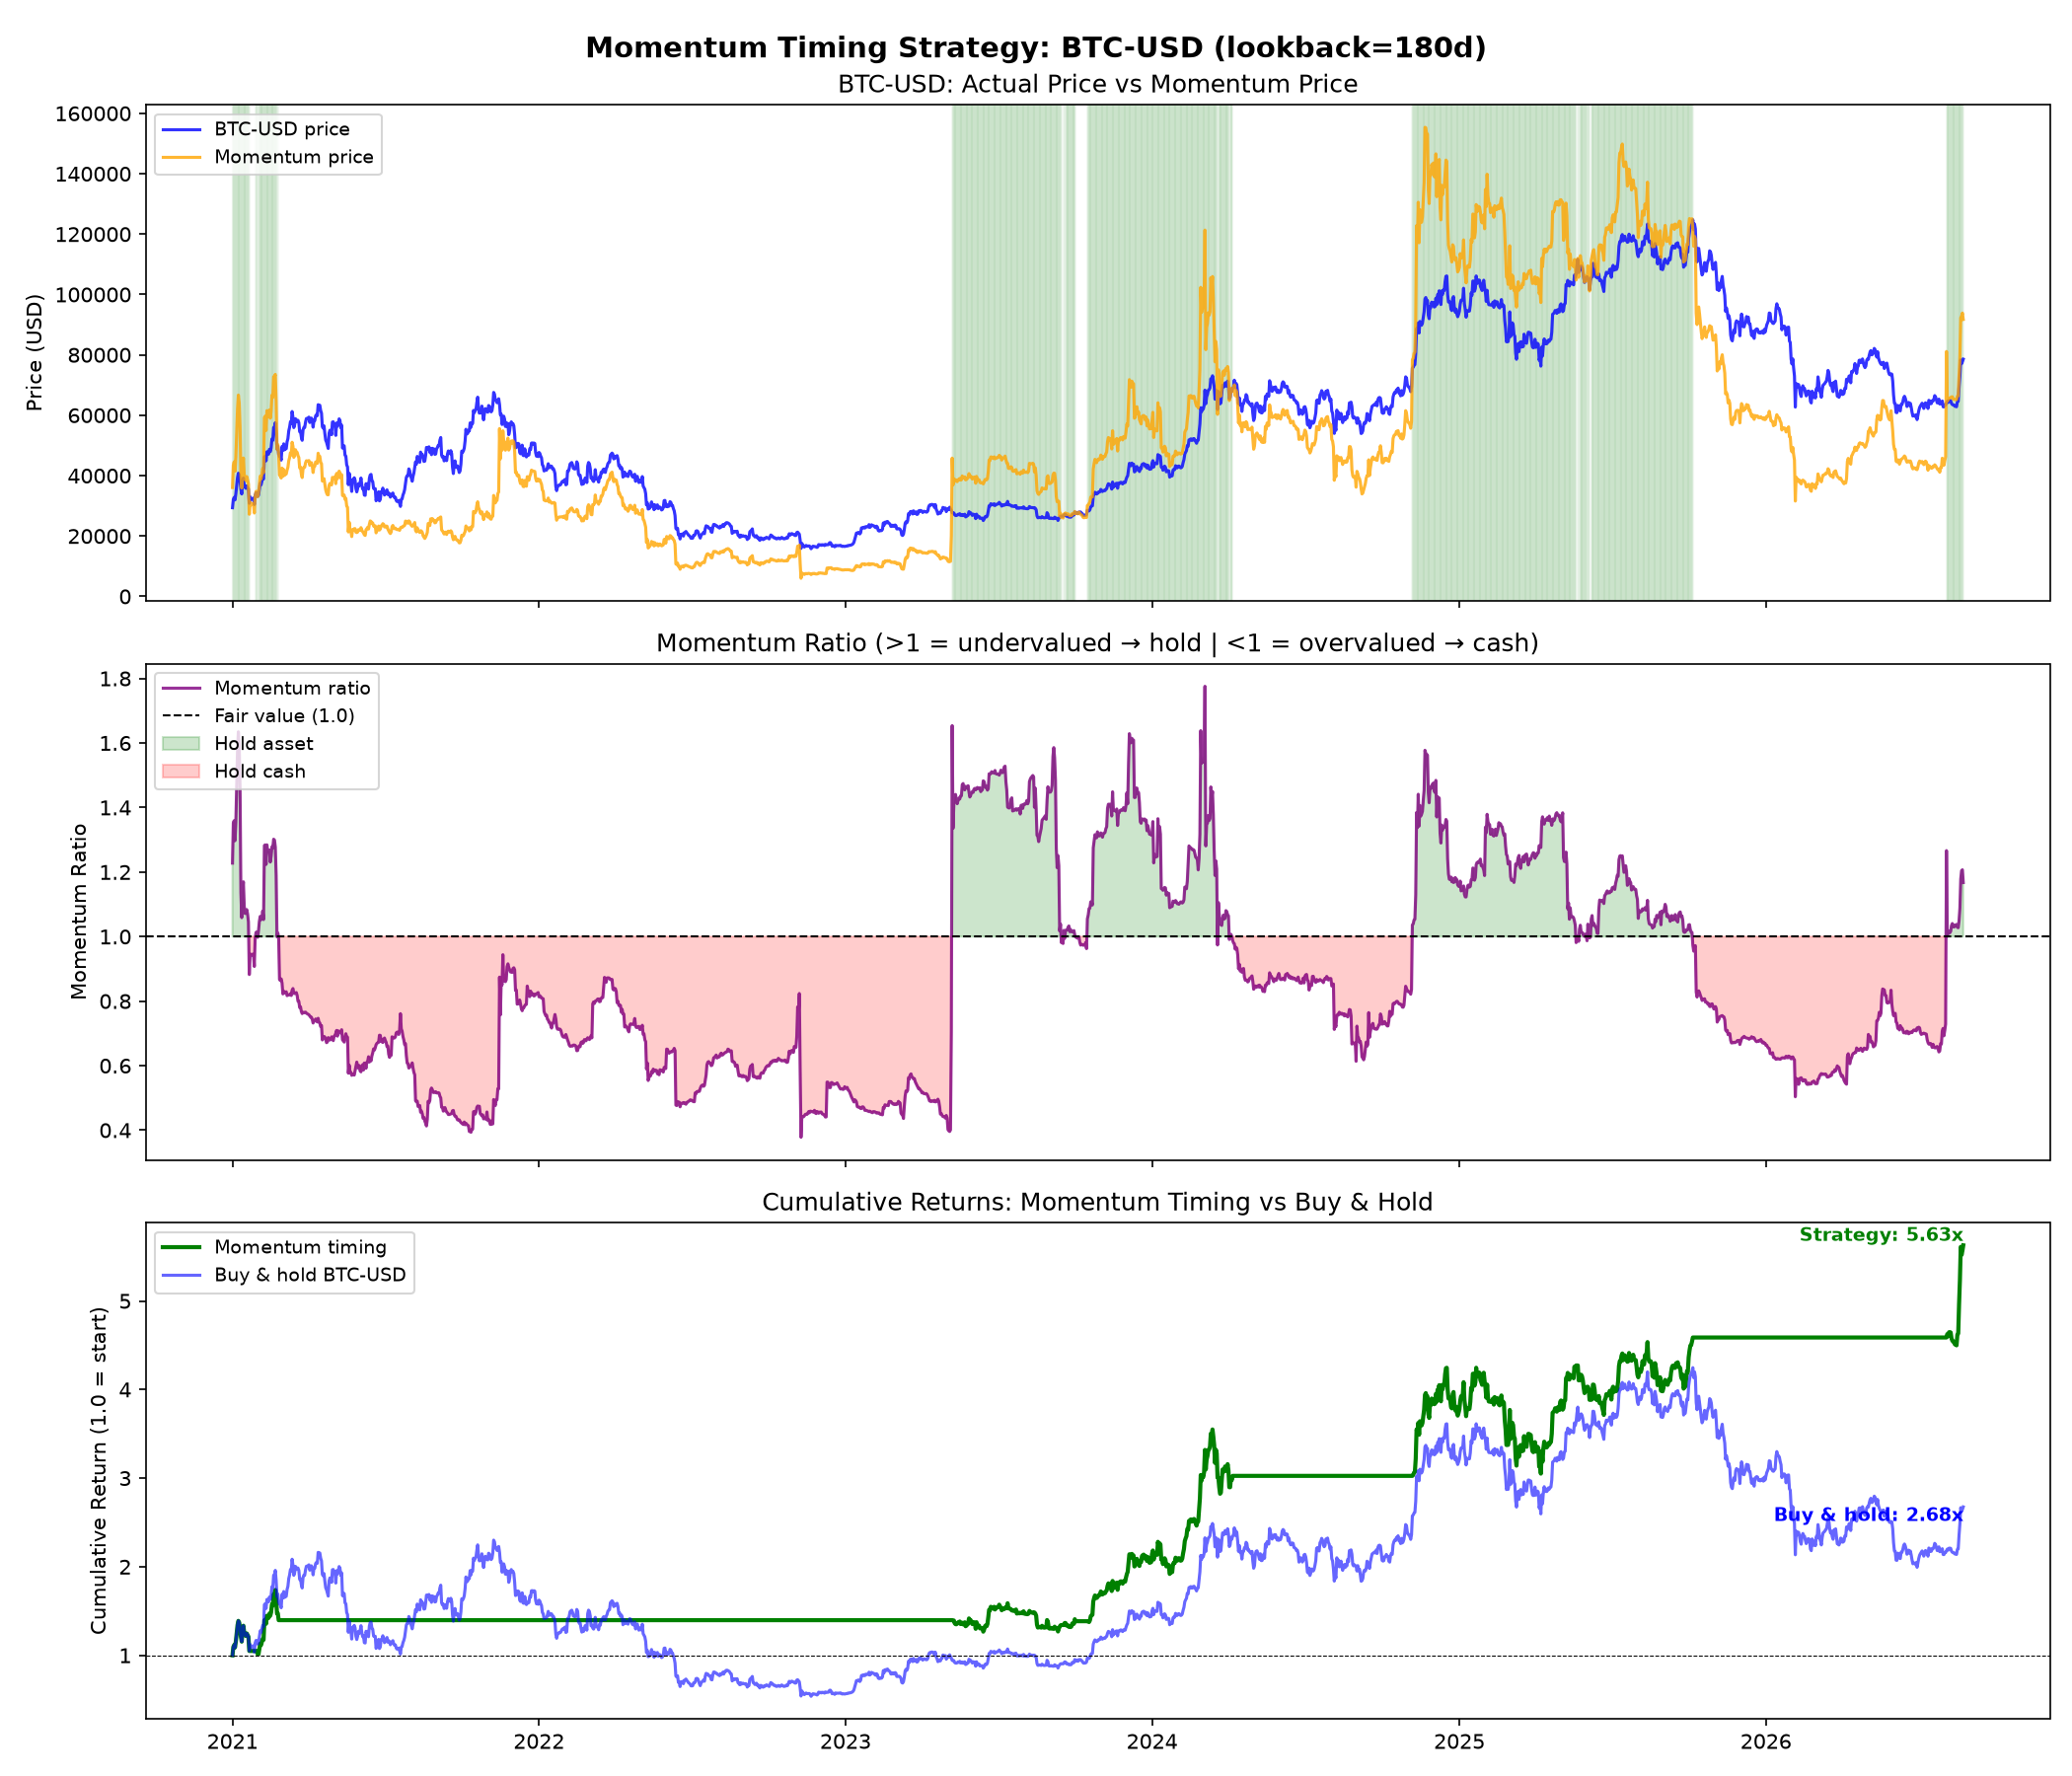
\includegraphics[width=\textwidth]{timing_BTCUSD.png}
    \caption{Bitcoin: the model exits before the 2022 crash,
    re-enters during the 2023 accumulation, and rides the
    2024--2025 bull run.}
\end{figure}

\begin{tcolorbox}[colback=blue!5, colframe=blue!40, boxrule=0.5pt, arc=3pt,
    left=6pt, right=6pt, top=4pt, bottom=4pt,
    title={\small\bfseries\color{blue!70} How to read the charts}]
{\small Each asset has a three-panel chart:
\begin{enumerate}[leftmargin=2em, topsep=2pt, itemsep=2pt]
    \item \textbf{Top --- Price vs Momentum Price.}
    Blue = actual price. Orange = \emph{momentum price}, a
    synthetic price from volume-weighted flow. Green shading
    marks days when the model says ``hold the asset.''

    \item \textbf{Middle --- Momentum Ratio.}
    Momentum price $\div$ actual price. Above the dashed line
    at 1.0: \textcolor{green}{\textbf{undervalued}} (hold asset).
    Below: \textcolor{red}{\textbf{overvalued}} (hold cash).
    The further from 1.0, the stronger the signal.

    \item \textbf{Bottom --- Cumulative Returns.}
    Green = strategy, blue = buy \& hold. Where green is above
    blue, the strategy is outperforming. Dips are drawdowns ---
    temporary losses before recovery.
\end{enumerate}}
\end{tcolorbox}

\subsection{Copper (HG=F, 180-day lookback)}

The quiet achiever. Copper has the highest Sharpe ratio among
commodity futures and a perfect win rate.

\vspace{0.5em}
\begin{tabular}{@{}lr@{}}
    \toprule
    \textbf{Metric} & \textbf{Value} \\
    \midrule
    Strategy return    & $+97.0\%$ \\
    Buy \& hold return & $+82.0\%$ \\
    Alpha              & $+15.0\%$ \\
    Sharpe ratio       & $1.05$ \\
    Max drawdown       & $-23.1\%$ (vs $-34.9\%$ buy \& hold) \\
    Win rate           & 100\% (6 trades) \\
    Avg win            & $+12.3\%$ \\
    Days in asset      & 35\% \\
    \bottomrule
\end{tabular}

\begin{figure}[H]
    \centering
    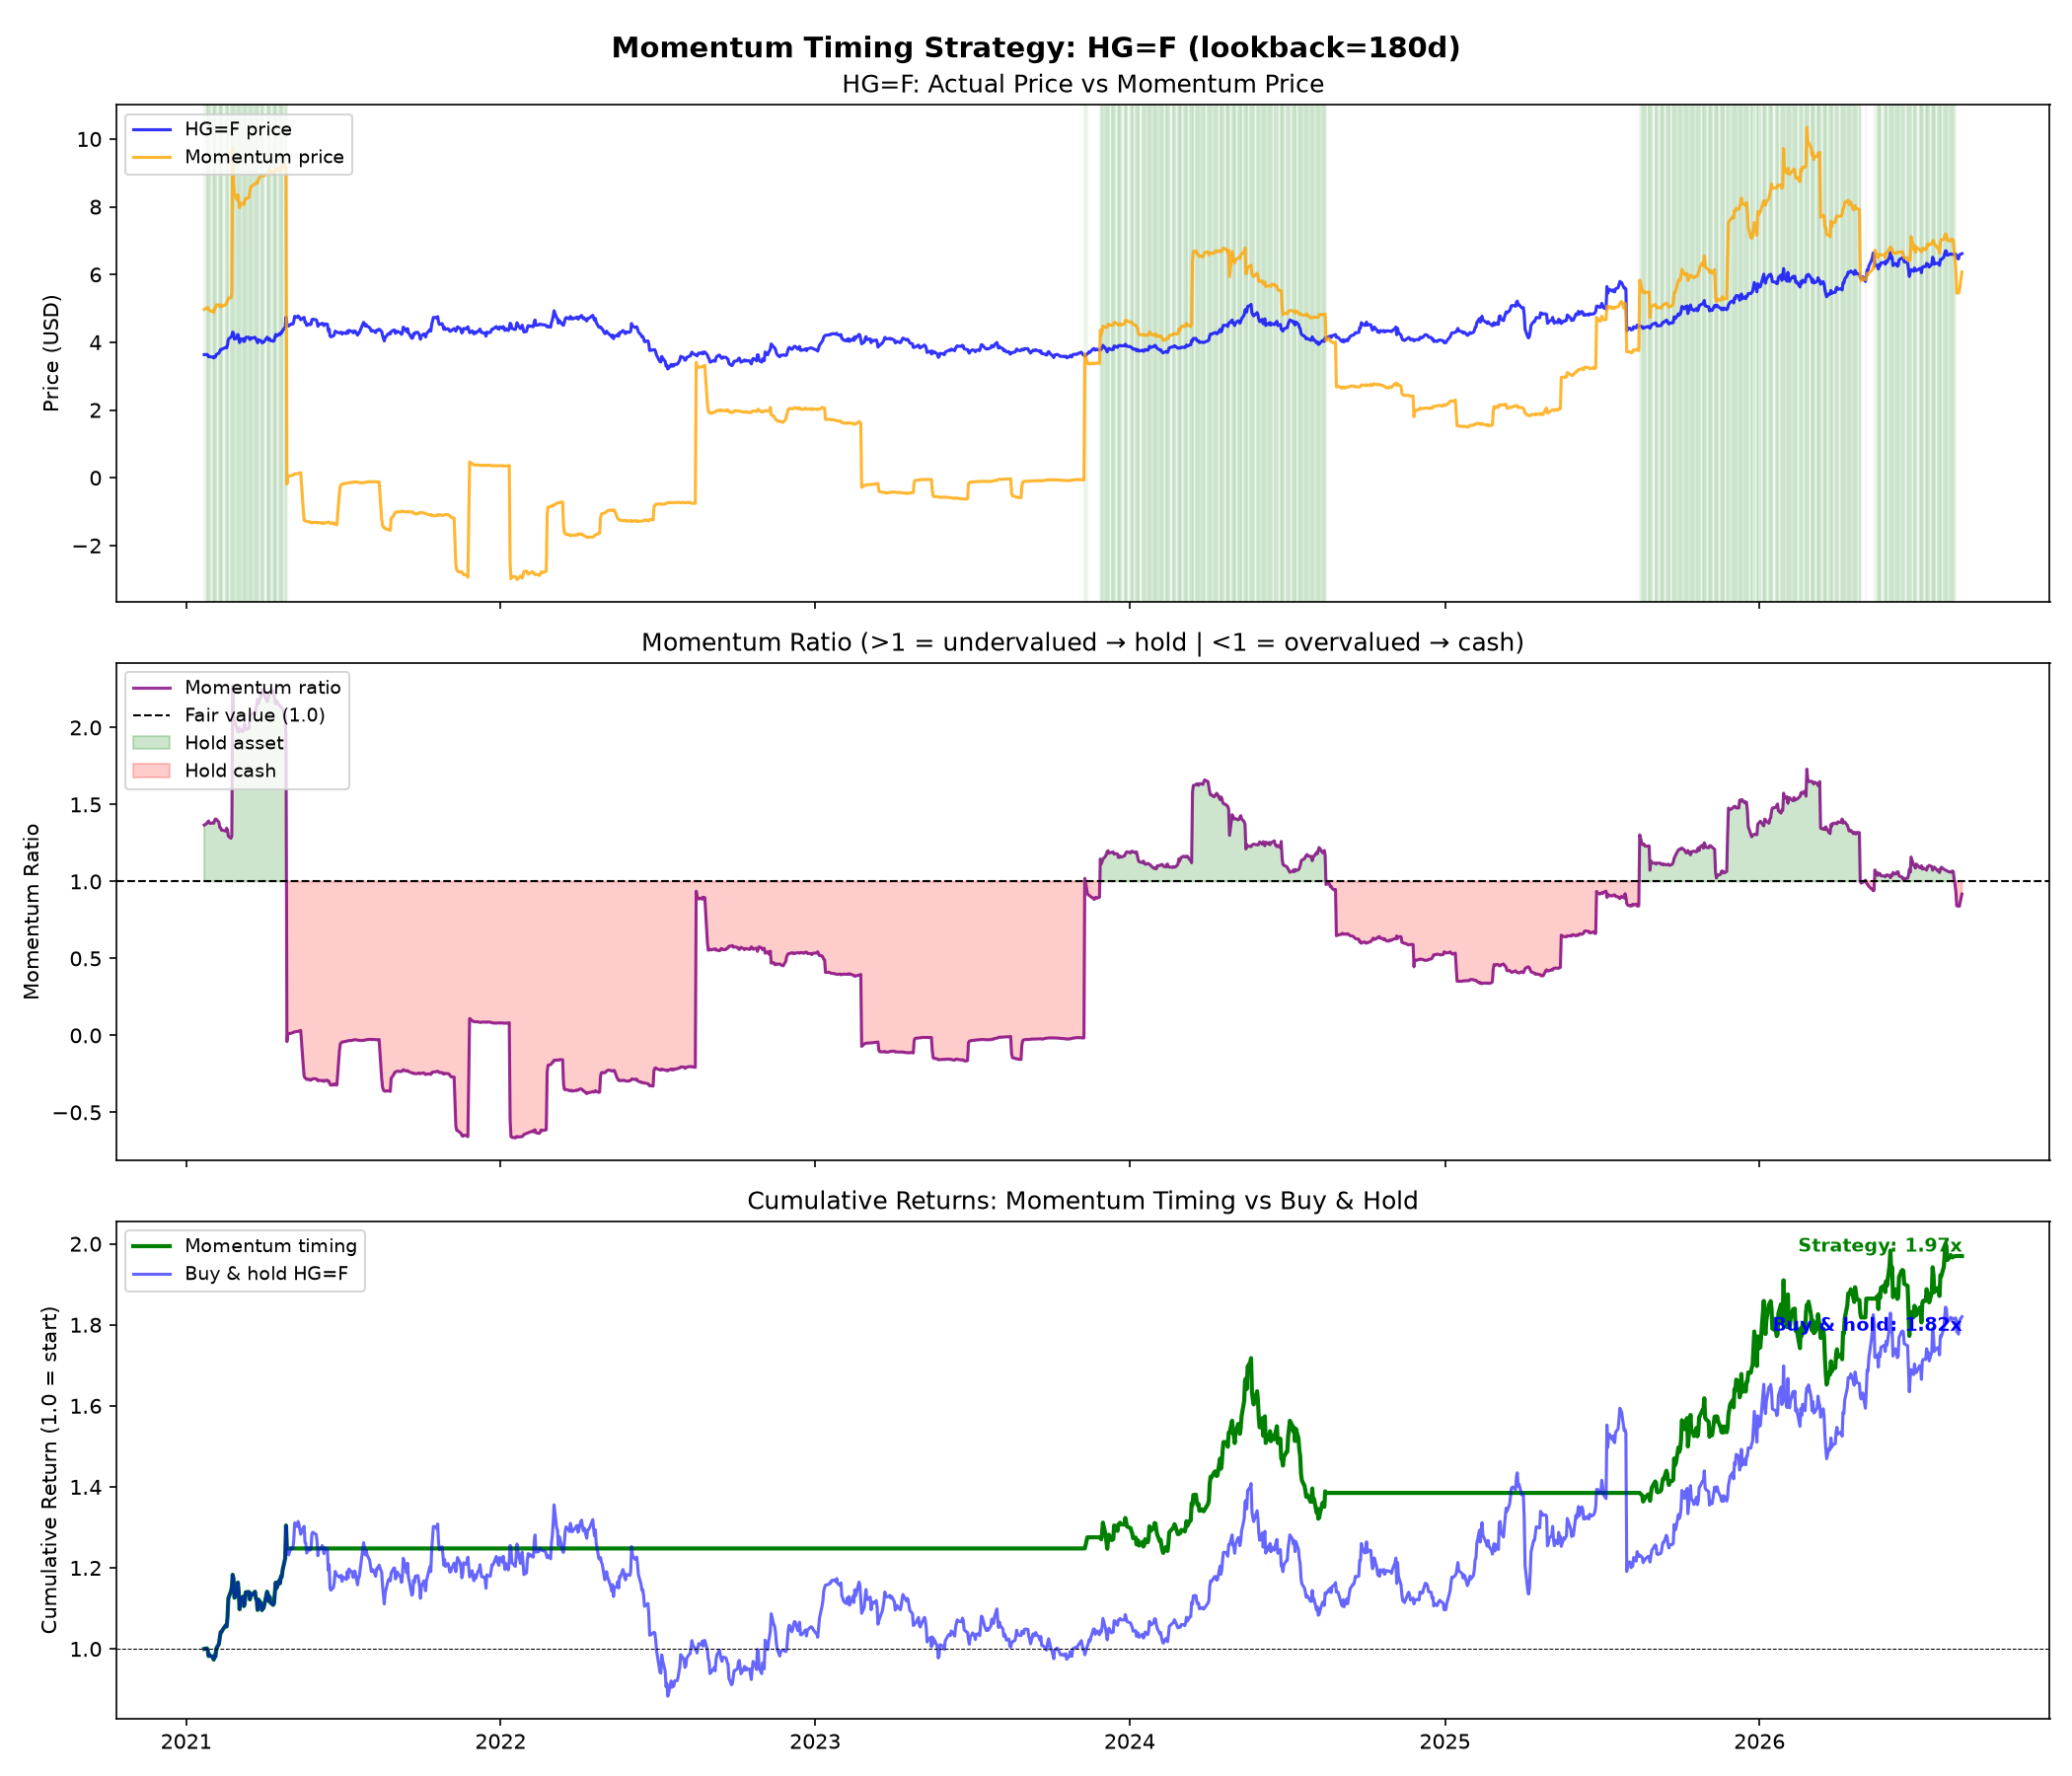
\includegraphics[width=\textwidth]{timing_HG=F.png}
    \caption{Copper: steady outperformance with minimal drawdown.
    The model catches the 2024--2025 commodity rally while avoiding
    the 2022 tightening-driven decline.}
\end{figure}




\subsection{Natural Gas (NG=F, 90-day lookback)}

The wildcard. Natural gas is the most volatile commodity tested,
and the \emph{only} asset where all three lookbacks (90, 180, 365
days) produce positive alpha. The 90-day lookback is optimal.

\vspace{0.5em}
\begin{tabular}{@{}lr@{}}
    \toprule
    \textbf{Metric} & \textbf{Value} \\
    \midrule
    Strategy return    & $+309.9\%$ \\
    Buy \& hold return & $+10.7\%$ \\
    Alpha              & \textcolor{green}{\textbf{+299.2\%}} \\
    Sharpe ratio       & $0.90$ \\
    Max drawdown       & $-53.0\%$ (vs $-83.7\%$ buy \& hold) \\
    Win rate           & 53\% (17 trades) \\
    Win/loss ratio     & 4.5:1 ($+25.6\%$ avg win vs $-5.7\%$ avg loss) \\
    Days in asset      & 50\% \\
    \bottomrule
\end{tabular}

\begin{figure}[H]
    \centering
    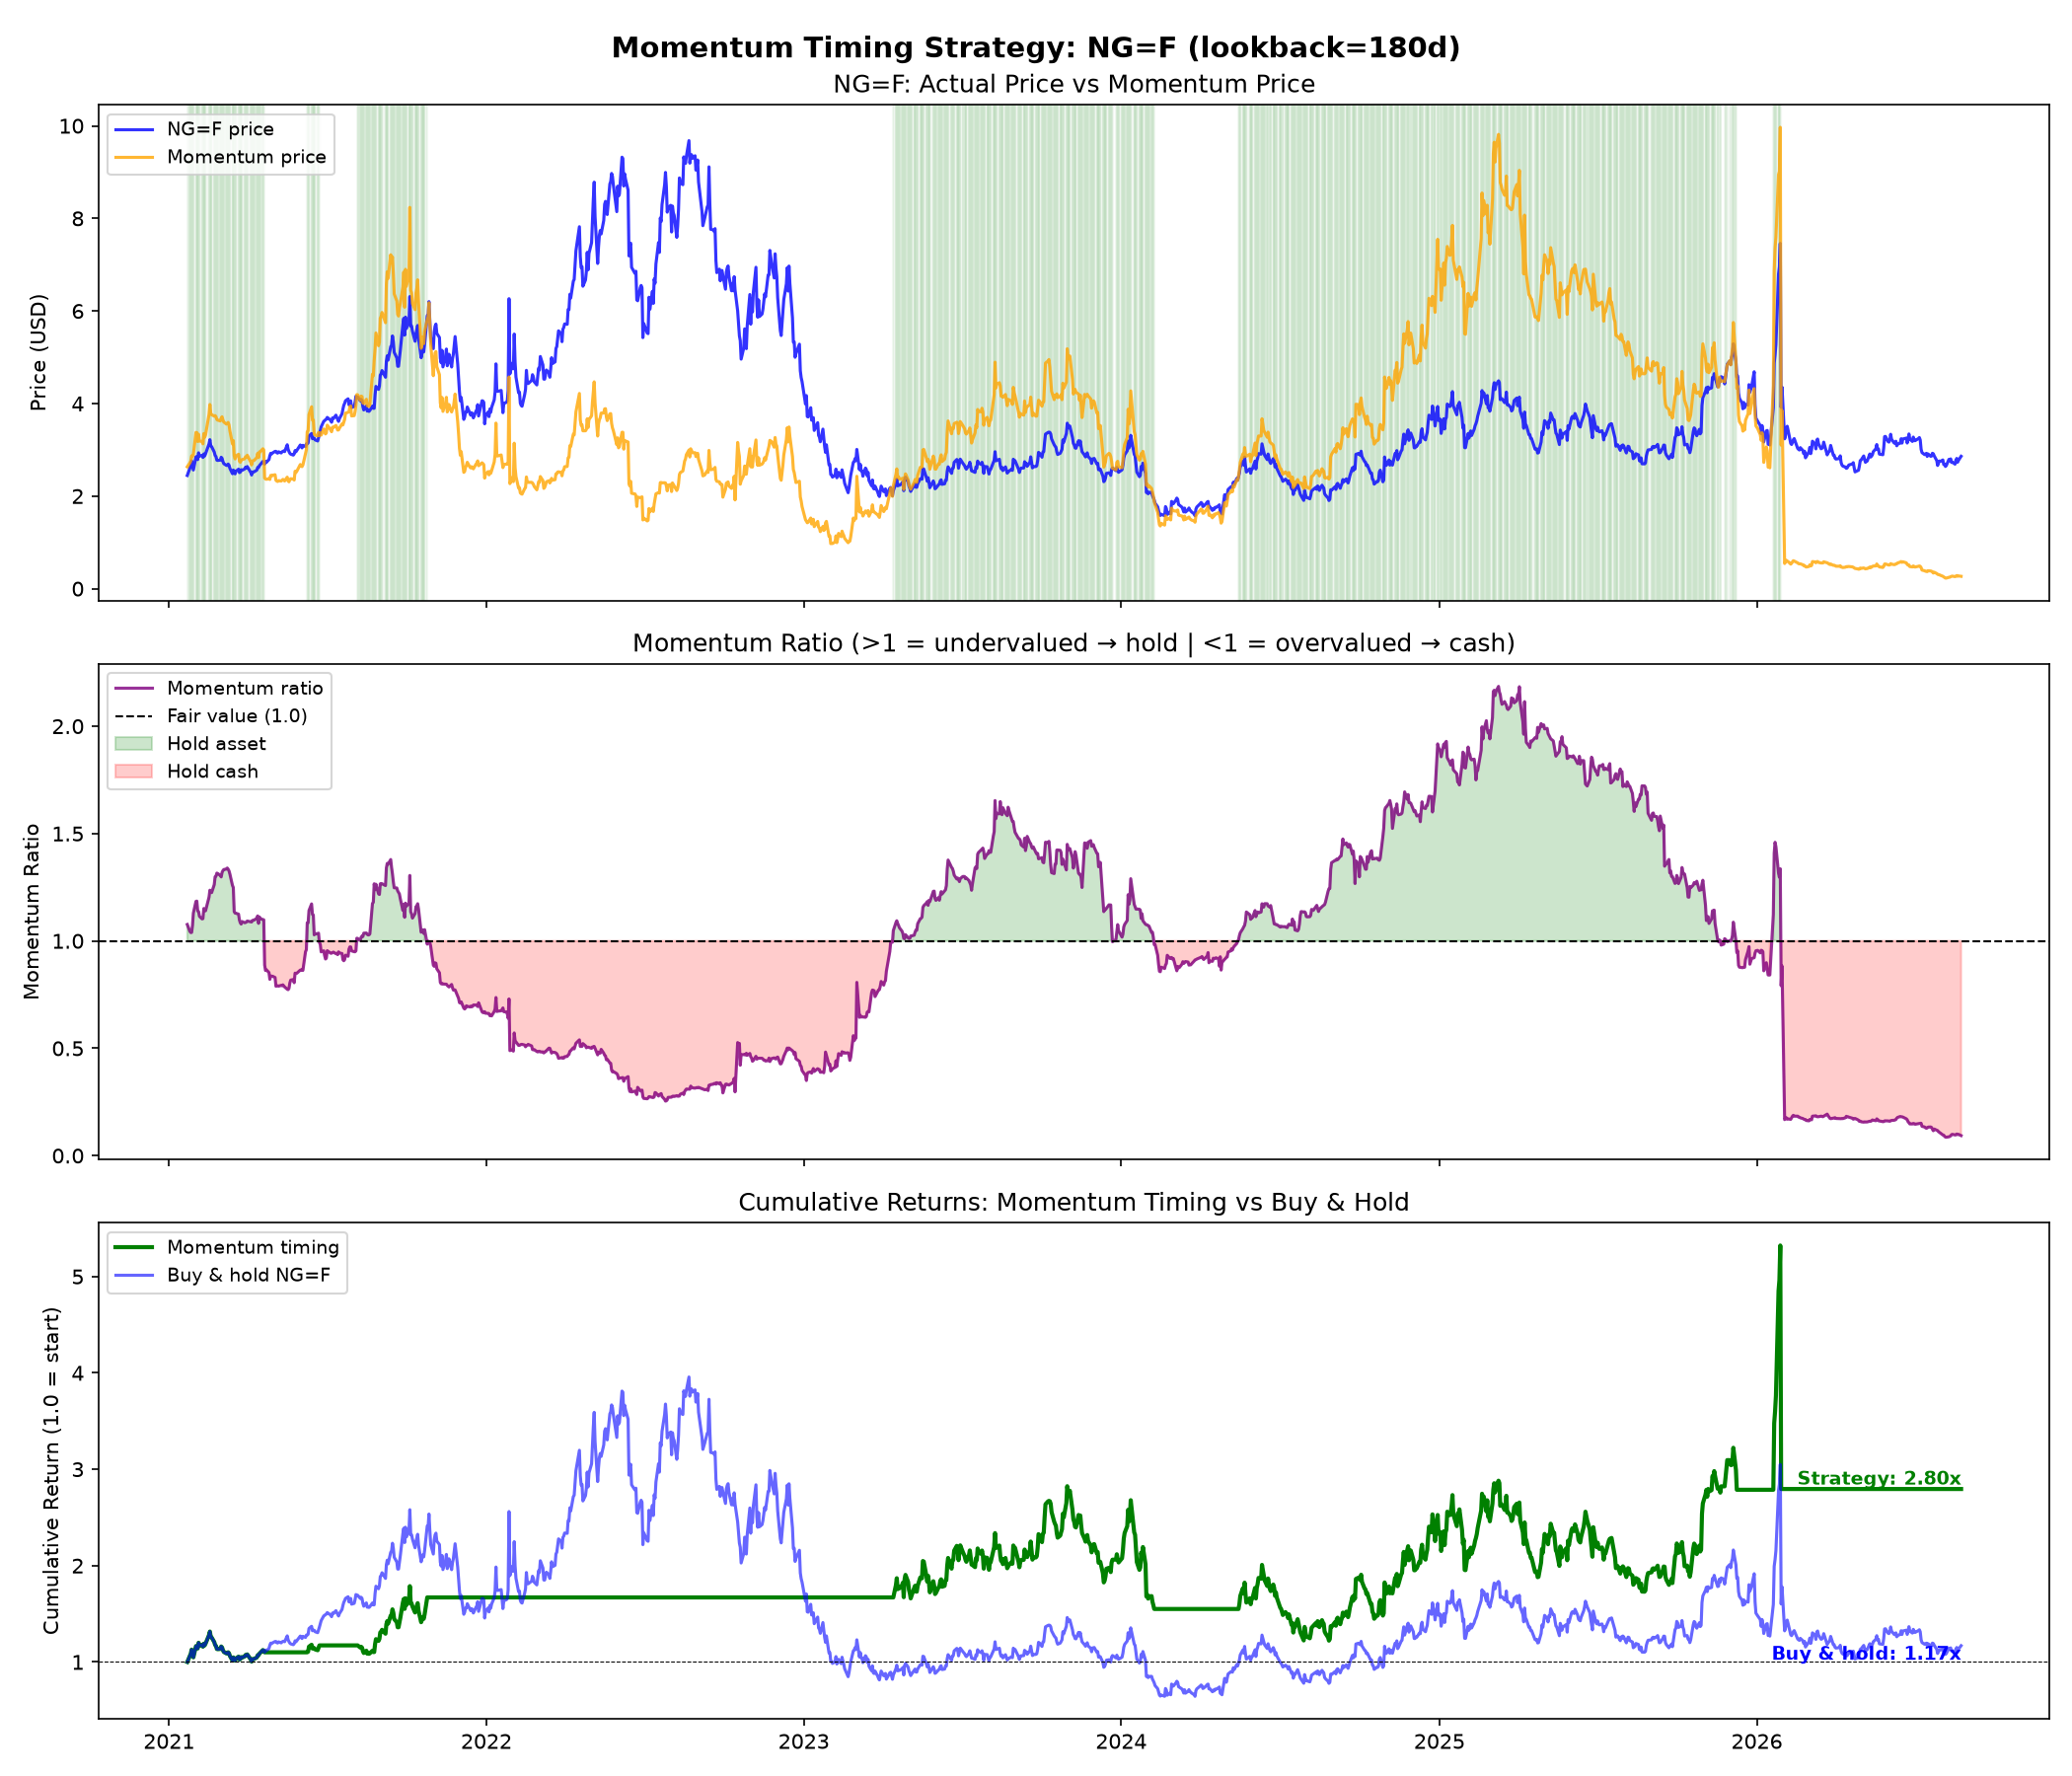
\includegraphics[width=\textwidth]{timing_NG=F.png}
    \caption{Natural gas: the model captures the 2021--2022 energy
    crisis spike and exits before the 83\% crash that followed.
    Buy \& hold returned only +11\% over 5 years; the strategy
    returned +310\%.}
\end{figure}




% ══════════════════════════════════════════════════════════════════
% EXECUTIVE SUMMARY
% ══════════════════════════════════════════════════════════════════




% ══════════════════════════════════════════════════════════════════
% THE RECYCLING IDEA
% ══════════════════════════════════════════════════════════════════

\section{The Capital Recycling Idea}

Pool all \$10,000 and allocate dynamically based on which assets
have active momentum signals:

\vspace{0.5em}
\begin{tabular}{@{}ll@{}}
    \toprule
    \textbf{Active assets} & \textbf{Allocation} \\
    \midrule
    3 assets active & 33\% / 33\% / 33\% \\
    2 assets active & 50\% / 50\% \\
    1 asset active  & 100\% in that asset \\
    0 assets active & 100\% cash \\
    \bottomrule
\end{tabular}

\vspace{0.5em}
When Bitcoin's signal says ``go to cash'' but copper's signal says
``hold,'' the money that \emph{would} have sat idle flows into
copper instead.

% ══════════════════════════════════════════════════════════════════
% RESULTS
% ══════════════════════════════════════════════════════════════════

\section{Results}

Period: 22 January 2021 to 24 August 2026 (1,406 trading days).
Starting capital: \$10,000.

\vspace{0.5em}
\begin{tabular}{@{}lr@{}}
    \toprule
    \textbf{Metric} & \textbf{Value} \\
    \midrule
    Final value  & \textcolor{green}{\textbf{\$108,003}} \\
    Total return  & \textcolor{green}{\textbf{+980\%}} \\
    Sharpe ratio  & $1.28$ \\
    Max drawdown  & $-35.3\%$ \\
    \bottomrule
\end{tabular}

\subsection{Capital Utilisation}

\vspace{0.5em}
\begin{tabular}{@{}lrr@{}}
    \toprule
    \textbf{State} & \textbf{Days} & \textbf{\% of time} \\
    \midrule
    0 assets active (100\% cash) & 368 & 26\% \\
    1 asset active               & 429 & 31\% \\
    2 assets active              & 580 & 41\% \\
    3 assets active              & 28  & 2\% \\
    \midrule
    \textbf{Capital deployed}    & \textbf{1,037} & \textbf{74\%} \\
    \bottomrule
\end{tabular}

\vspace{0.5em}
Compare this to individual assets, which are deployed only
34--50\% of the time. The recycling portfolio has capital
working \textbf{74\% of the time}.

\subsection{Portfolio Equity Curve}

\begin{figure}[H]
    \centering
    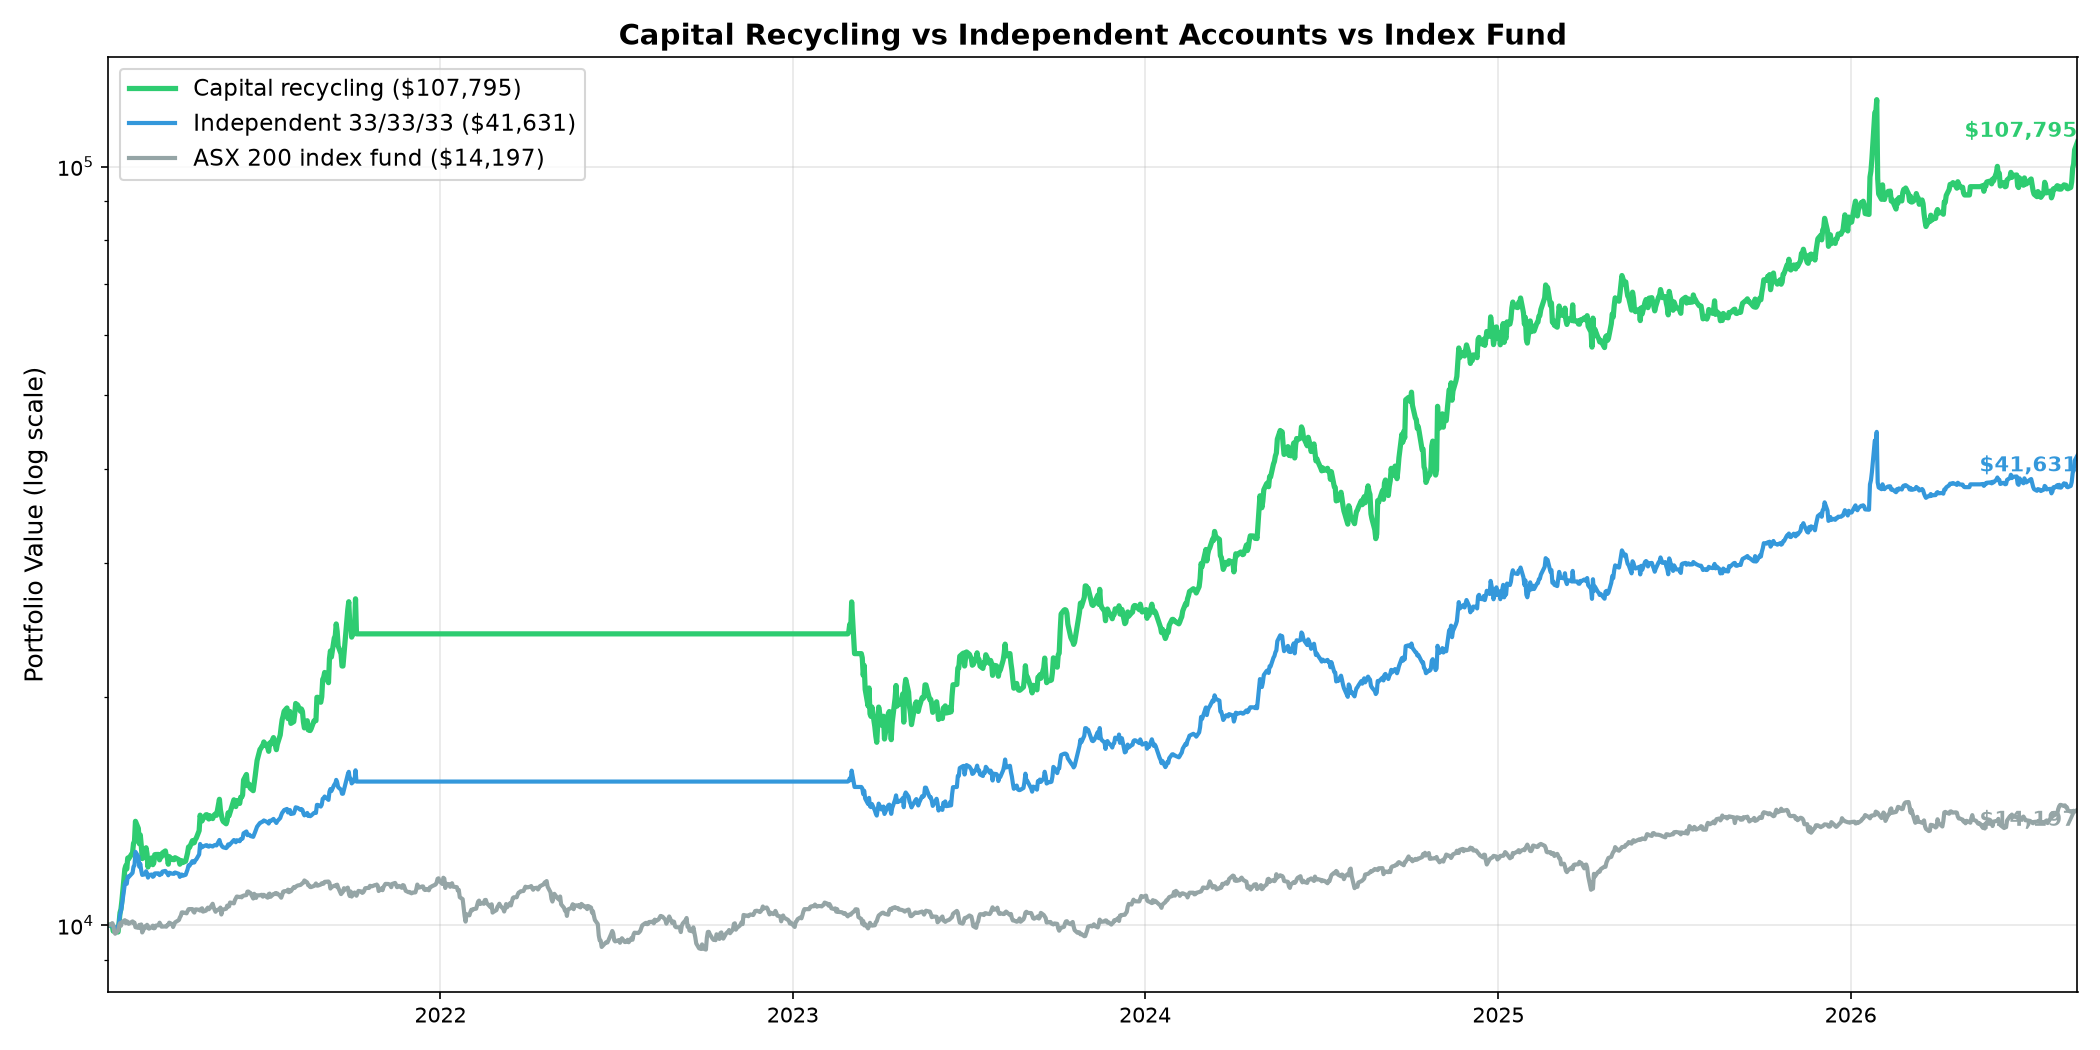
\includegraphics[width=\textwidth]{portfolio_comparison.png}
    \caption{Capital recycling vs running three independent accounts
    vs the ASX 200 index fund (log scale). Recycling turns \$10,000
    into \$108,003 by keeping idle capital deployed.}
\end{figure}




% ══════════════════════════════════════════════════════════════════
% CAVEATS
% ══════════════════════════════════════════════════════════════════

\section{Caveats}

\begin{enumerate}[leftmargin=2em]
    \item \textbf{Backtest $\neq$ live trading.} These results assume
          execution at the daily close with no slippage, fees, or
          bid-ask spreads.

    \item \textbf{Small sample sizes.} 6--17 trades per asset over
          5 years is not statistically robust. Strong alpha may be
          driven by a few large wins.

    \item \textbf{No transaction costs.} Crypto exchange fees
          (0.1--0.5\%), futures commissions, and the bid-ask spread
          on commodity futures will reduce returns. The recycling
          model rebalances frequently, amplifying this cost.

    \item \textbf{Tax drag.} Each trade is a taxable event.
          Frequent rebalancing creates short-term capital gains.

    \item \textbf{Volume data quality.} Crypto volumes may be
          inflated by wash trading. Commodity futures volumes from
          yfinance are a fraction of actual CME volumes.

    \item \textbf{Execution complexity.} The recycling model requires
          simultaneous positions in crypto (24/7 markets) and commodity
          futures (exchange hours only). Rebalancing across asset
          classes adds operational risk.

    \item \textbf{Survivor bias.} We selected these three assets
          \emph{because} they showed strong momentum alpha. An
          out-of-sample test is essential before committing real capital.
\end{enumerate}




\newpage
\begin{resultbox}[]{warn}
\begin{center}
\Large\bfseries Historical returns do not guarantee future returns.
\end{center}

\vspace{0.5em}
The results in this report are based on backtested simulations
using historical data from January 2021 to August 2026. Past
performance is not indicative of future results. Market conditions,
volume dynamics, and correlations between assets can and do change.
The bookmaker-pool model may stop working if the volume--price
dynamics that produced these signals evolve.

\vspace{0.5em}
Before committing real capital, paper trade the strategy for at
least 3--6 months to verify that the signals remain actionable in
live market conditions.
\end{resultbox}




% ══════════════════════════════════════════════════════════════════
% APPENDIX: SOURCE CODE
% ══════════════════════════════════════════════════════════════════

\appendix

\section{Source Code}

All code lives in \texttt{$\sim$/git/andy/crypto/}. Python 3.8+,
no exchange account needed for backtesting.

\subsection{Setup}

\begin{codebox}[Shell]
\begin{lstlisting}[style=shell]
cd ~/git/andy/crypto
python3 -m venv venv
source venv/bin/activate
pip install yfinance pandas numpy matplotlib
\end{lstlisting}
\end{codebox}

\subsection{Running the Individual Backtests}

\begin{codebox}[Shell]
\begin{lstlisting}[style=shell]
# Bitcoin (180-day lookback)
python momentum_single.py --asset BTC-USD \
       --lookback 180 --start 2021-01-01 --plot

# Copper (180-day lookback)
python momentum_single.py --asset HG=F \
       --lookback 180 --start 2021-01-01 --plot

# Natural Gas (90-day lookback)
python momentum_single.py --asset NG=F \
       --lookback 90 --start 2021-01-01 --plot
\end{lstlisting}
\end{codebox}

\subsection{momentum\_single.py}

The individual asset backtests. Implements the bookmaker-pool
momentum model and the timing simulation.

\begin{codebox}[momentum\_single.py]
\begin{lstlisting}[style=python]
"""
Crypto momentum timing: single-asset directional
strategy.

Uses the bookmaker-pool momentum model to time
entries and exits. Hold when momentum price > actual
price; go to cash when momentum price < actual price.

Usage:
  python momentum_single.py
  python momentum_single.py --asset HG=F
  python momentum_single.py --lookback 90 --plot
"""

import argparse, os
import numpy as np
import pandas as pd
import yfinance as yf
from datetime import datetime, timedelta
import matplotlib
matplotlib.use("Agg")
import matplotlib.pyplot as plt

SCRIPT_DIR = os.path.dirname(
    os.path.abspath(__file__))


def compute_rolling_momentum(history, lookback_days):
    """
    Rolling momentum price via the bookmaker pool.

    Volume is normalised (divided by window mean) to
    prevent overflow on crypto's enormous volumes.
    """
    closes = history["Close"].values
    volumes = history["Volume"].values
    dates = history.index

    momentum_prices = [np.nan] * len(history)
    momentum_ratios = [np.nan] * len(history)

    for i in range(lookback_days, len(history)):
        window_close = closes[
            i - lookback_days:i + 1]
        window_vol = volumes[
            i - lookback_days:i + 1]

        if len(window_close) < 10:
            continue

        returns = (np.diff(window_close)
                   / window_close[:-1])
        vols = window_vol[1:]

        mean_vol = vols.mean()
        if mean_vol == 0:
            continue
        norm_vols = vols / mean_vol

        # Net flow = normalised_volume * return
        net_flows = norm_vols * returns

        # Run the bookmaker pool
        pool = float(window_close[0])
        mp = pool
        for j in range(len(net_flows)):
            pool += net_flows[j] * mp
            mp = pool

        momentum_prices[i] = mp
        momentum_ratios[i] = mp / closes[i]

    result = pd.DataFrame({
        "Close": closes,
        "MomentumPrice": momentum_prices,
        "MomentumRatio": momentum_ratios,
    }, index=dates)

    return result.dropna()


def simulate_timing(asset_symbol, lookback_days,
                    start_date, end_date):
    """
    Simulate the timing strategy.

    Rule:
      MomentumRatio > 1.0 -> hold asset
      MomentumRatio <= 1.0 -> hold cash
    """
    fetch_start = start_date - timedelta(
        days=lookback_days + 60)

    ticker = yf.Ticker(asset_symbol)
    hist = ticker.history(
        start=fetch_start, end=end_date,
        interval="1d")

    if hist.empty:
        raise ValueError(
            f"No data for {asset_symbol}")

    df = compute_rolling_momentum(
        hist, lookback_days)

    # Trim to simulation period
    start_ts = pd.Timestamp(start_date)
    if df.index.tz is not None:
        start_ts = start_ts.tz_localize(
            df.index.tz)
    df = df[df.index >= start_ts]

    # Signals: 1 = hold asset, 0 = hold cash
    df["signal"] = (
        df["MomentumRatio"] > 1.0).astype(int)

    # Position: use previous day's signal
    df["position"] = (
        df["signal"].shift(1).fillna(0).astype(int))

    # Returns
    df["asset_return"] = (
        df["Close"].pct_change().fillna(0))
    df["strategy_return"] = (
        df["position"] * df["asset_return"])

    # Cumulative
    df["cumulative_asset"] = (
        1 + df["asset_return"]).cumprod()
    df["cumulative_strategy"] = (
        1 + df["strategy_return"]).cumprod()

    return df
\end{lstlisting}
\end{codebox}




\subsection{portfolio\_recycling.py}

The three-asset recycling portfolio simulation.

\begin{codebox}[portfolio\_recycling.py]
\begin{lstlisting}[style=python]
"""
Three-asset recycling portfolio.

When an asset's momentum signal says "cash", its
capital flows to whichever other assets are active.
"""

import numpy as np
import pandas as pd
import yfinance as yf
import matplotlib
matplotlib.use("Agg")
import matplotlib.pyplot as plt
from datetime import datetime
from momentum_single import simulate_timing

ASSETS = [
    ("BTC-USD", 180),  # (ticker, lookback_days)
    ("HG=F",   180),   # copper
    ("NG=F",    90),   # natural gas
]
START = datetime(2021, 1, 1)
END   = datetime(2026, 8, 25)
CAPITAL = 10_000


def run_portfolio():
    # Run individual backtests
    sims = {}
    for ticker, lookback in ASSETS:
        sims[ticker] = simulate_timing(
            ticker, lookback, START, END)

    # Align to common dates (futures calendar)
    futures = [
        t for t, _ in ASSETS if "USD" not in t]
    common = sims[futures[0]].index
    for t in futures[1:]:
        common = common.intersection(
            sims[t].index)

    aligned = {}
    for ticker, _ in ASSETS:
        if "USD" in ticker:
            aligned[ticker] = sims[
                ticker].reindex(
                    common, method="ffill")
        else:
            aligned[ticker] = sims[
                ticker].loc[common]

    n_days = len(common)
    n_assets = len(ASSETS)

    signals = np.column_stack([
        aligned[t]["position"].values
        for t, _ in ASSETS])
    returns = np.column_stack([
        aligned[t]["asset_return"].values
        for t, _ in ASSETS])

    # Simulate recycling portfolio
    portfolio = np.ones(n_days)
    daily_rets = np.zeros(n_days)

    for i in range(1, n_days):
        active = [
            j for j in range(n_assets)
            if signals[i, j] == 1]
        if not active:
            daily_rets[i] = 0.0
        else:
            w = 1.0 / len(active)
            port_ret = sum(
                w * returns[i, j]
                for j in active)
            daily_rets[i] = port_ret

        portfolio[i] = portfolio[i-1] * (
            1 + daily_rets[i])

    final = CAPITAL * portfolio[-1]

    # Risk metrics
    cummax = np.maximum.accumulate(portfolio)
    dd = (portfolio - cummax) / cummax
    max_dd = dd.min() * 100
    sharpe = (np.mean(daily_rets[1:])
              / np.std(daily_rets[1:])
              * np.sqrt(252))

    print(f"${CAPITAL:,} -> ${final:,.0f} "
          f"(+{(final/CAPITAL-1)*100:.0f}%)")
    print(f"Sharpe:  {sharpe:.2f}")
    print(f"Max DD:  {max_dd:.1f}%")

    return common, portfolio, signals, aligned


if __name__ == "__main__":
    run_portfolio()
\end{lstlisting}
\end{codebox}

\vspace{2em}
\begin{center}
\textit{--- Robin}
\end{center}

\end{document}
